\begin{center}
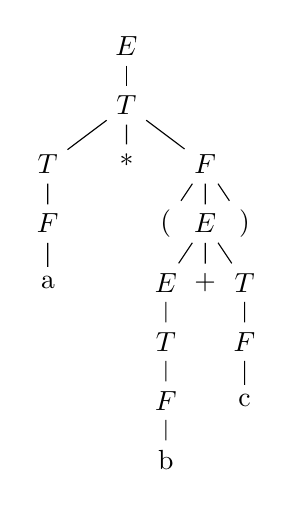
\begin{tikzpicture}[
    level distance=0.75cm,
    level 2/.style={sibling distance=1cm},
    level 3/.style={sibling distance=0.5cm}
]
    \node {$E$}
    child {node {$T$}
        child {node {$T$}
            child {node{$F$}
                child{node{\str{a}}}
            }
        }
        child {node {\str{*}}}
        child {node {$F$}
            child {node{\str{(}}}
            child {node {$E$}
                child {node {$E$}
                    child {node {$T$}
                        child {node{$F$}
                            child{node{\str{b}}}
                        }
                    }
                }
                child {node {\str{+}}}
                child {node {$T$}
                    child {node{$F$}
                        child{node{\str{c}}}
                    }
                }
            }
            child {node{\str{)}}}
        }
    };
\end{tikzpicture}
\end{center}